


\subsection{Funktionsstruktur und Konzeptbewertung}

Ein Konzept stellt in erster Linie einen prinzipiellen Aufbau dar und dient der Überprüfung, inwieweit die gestellten Anforderungen erfüllt wurden. Da durch das Konzept die grundlegende Gestalt und die wichtigsten Merkmale festgelegt werden, ist die Konzeptphase einer der wichtigsten Abschnitte im Entwicklungsprozess. Das Gesamtkonzept lässt sich nach~\cite{Pahl_Beitz_Konstruktionslehre} folgendermaßen unterteilen:

\begin{description}
    \item[Gestaltungskonzept] Festlegung der grundlegenden Geometrie, Zuordnung der einzelnen Komponenten und Betrachtung von Stoff-, Energie- und Signalflüssen
    \item[Wirkkonzept] Beschreibung der physikalischen Effekte und deren Verknüpfung zur Erfüllung der gestellten Anforderungen sowie der Gestalt der Wirkflächen
    \item[Wirkfläche] Funktionale Flächen, an denen das Wirkkonzept umgesetzt wird
\end{description}

Unter Berücksichtigung der Forderungen, welche die Funktion unmittelbar beeinflussen, wurden zunächst die wesentlichen Aufgaben der Konstruktion identifiziert. Die Gesamtaufgabe ist bereits eindeutig festgelegt: Innerhalb einer von äußeren Störeinflüssen abgeschirmten Messkabine sollen Probekörper im Koppelpfad zweier Hornantennen positioniert werden, wobei durch die geometrischen Abmessungen und die Verkleidung reflektiver Flächen im Inneren der Messkammer sichergestellt werden soll, dass sich die Proben im ungestörten Fernfeld (vgl. \Kapitel\ref{cha:2}) der Antennen befinden. Festzulegen bleibt im Weiteren der genaue Aufbau der Messkabine unter Berücksichtigung der zu erreichenden Schirmung, die Gestaltung von Öffnungen und Durchführungen, die Positionierung der Antennen und Probekörper und die Auswahl geeigneter Absorber, um Hohlraumresonanzen (vgl. \Abschnitt\ref{cha:2_subsub_Hohlraumresonanzen}), Reflektionen und indirekte Kopplung (vgl. \Abschnitt\ref{cha:2_sub_Reflektion}) zu vermeiden. Mithilfe der in \Abb\ref{fig:3_Funktionsstruktur} dargestellten Funktionsstruktur wurde die Gesamtaufgabe weiter abstrahiert und gegliedert. %Die Qualifikation des Teststandes anhand des Vergleiches der durchgeführten und mit früheren Messungen ist als Teil der Auswertung nicht in der Funktionsstruktur enthalten.

\begin{figure}[ht]
    \centering
    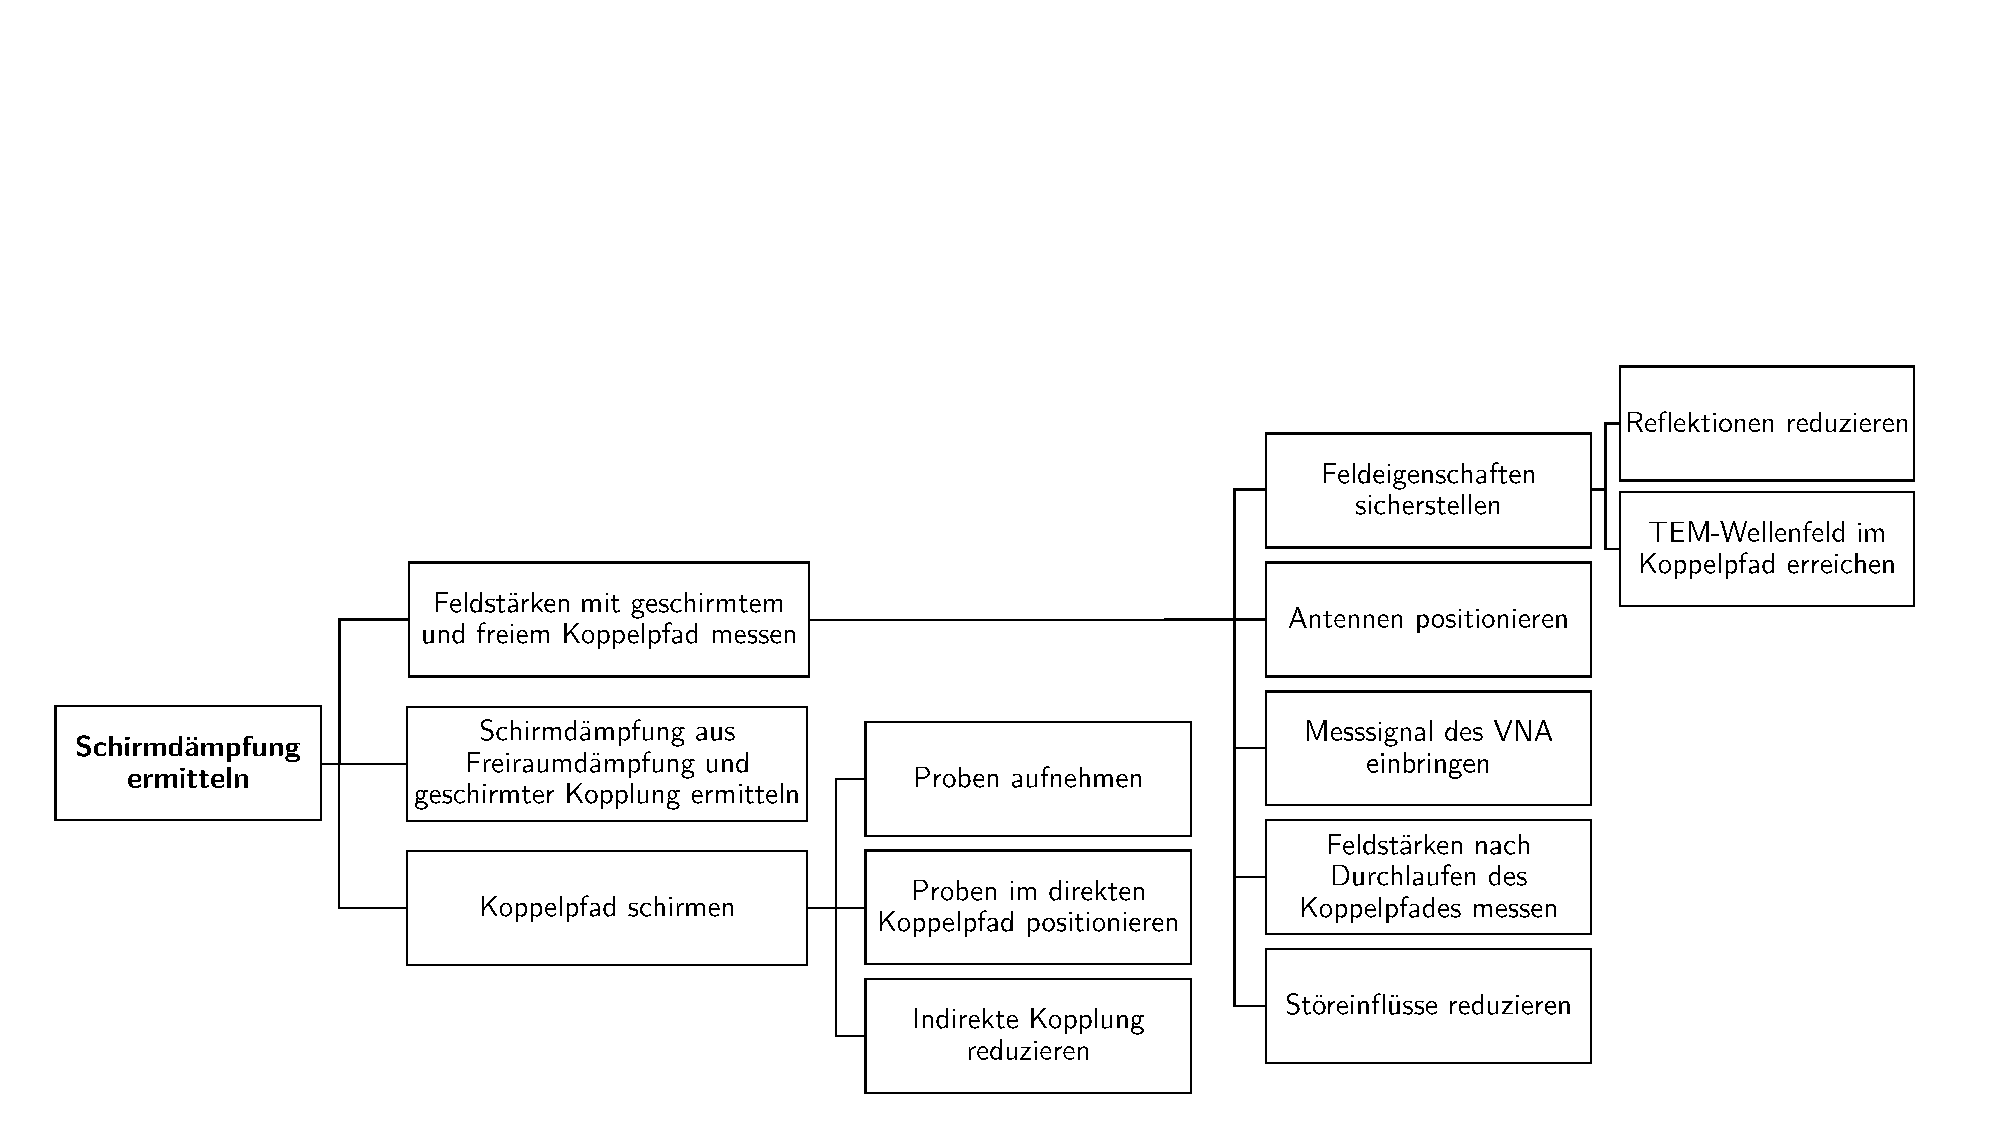
\includegraphics[page = 1, width=\textwidth, trim = 0.8cm 0.5cm 1.3cm 5.5cm, clip]{Abbildungen/Kapitel3/Funktionsstruktur.pdf}
    \caption{Funktionsstruktur der Messkabine}
    \label{fig:3_Funktionsstruktur}
\end{figure}


Auf dieser Grundlage lassen sich nun verschiedene Wirkkonzepte für die Teilstrukturen der Messkammer und deren Wirkflächen erstellen. Das Augenmerk des Designs lag dabei auf einer robusten und einfachen Geometrie der Wirkflächen bei gleichzeitiger Gewährleistung einer möglichst hohen Dichtheit gegenüber elektromagnetischer Strahlung. Letzteres kann nach der betrachteten Theorie in den \Abschnitten\ref{cha:2_sub_Daempfung_und_Absorption}, \ref{cha:2_sub_Reflektion} und \ref{cha:2_sub_Schirmung_ebener_Wellenfelder} durch die Herstellung eines leitfähigen Flächenkontaktes mit möglichst geringem Kontaktwiderstand zwischen allen Elementen der äußeren Schirmwand erreicht werden. Dies ist somit der physikalische Effekt, auf dem die Wirkkonzepte der Messkabine und der Durchführungen beruhen. 
\par
\vspace{\linespace}
Zur strukturierten und nachvollziehbaren Durchführung des Entscheidungsprozesses und der Auswahl der potenziell besten aus den vorgestellten Lösungsvarianten, kam ein Bewertungsschema zum Einsatz. Die Bewertungskriterien wurden nach dem Top-down-Vorgehen abgeleitet. Das beudeutet die Anforderungen des gesamten Versuchsstandes wurden für die einzelnen Teilsysteme detailliert~\cite{Pahl_Beitz_Konstruktionslehre}. Die gewählten Kriterien weisen die in~\cite{Pahl_Beitz_Konstruktionslehre} beschriebenen Voraussetzungen, wie unter anderem Freiheit von Dopplungen, Gegenläufigkeit und Widersprüchen sowie Gültigkeit für alle vorgestellten Varianten, auf.
\par
\vspace{\linespace}
Die Bewertung bestand aus der Anwendung eines gewichteten Punkteschemas, welches allen Kriterien Maßzahlen hinsichtlich ihrer Erfüllung durch die Konzepte zuordnete. Dies sorgte für ein vergleichsweise einfaches Bewertungsschema, welches gegenüber einer reinen Argumentenbilanz jedoch eine deutlich präzisere Entscheidung zulässt und die quantifizierbare Möglichkeit einer Wichtung bietet. Die Bewertung der einzelnen Konzepte erfolgte getrennt je Teilsystem des Aufbaus. Mithilfe des errechneten Gesamtwertes $G_V$ je Lösungsvariante aus den Maßzahlen $M$ und den Gewichtet $w$ konnte die Auswahl der besten Variante unmittelbar erfolgen~\cite{Pahl_Beitz_Konstruktionslehre}:

\begin{equation}
    G_{V_i} = \sum_{j=1}^{k} w_j \cdot M_{j,i}
    \label{eq:3_Gesamtwert_Variantenvergleich}
\end{equation}
\begin{equation}
    w_j \in \{\mathbb{Q} \;\vert\; 0 < w_j \leq 1\}; \qquad \sum_{j=1}^{k} w_j = 1; \qquad M_{j,i} \in \{1,\,2,\,3,\,4\}
    \label{eq:3_Wichtung_Bewertung}
\end{equation}
\begin{equation*}
    \text{\textit{k: Anzahl Kriterien; i: Variante; j: Kriterium}}
\end{equation*}

Eine höhere Maßzahl der Bewertung steht dabei stets für die jeweils bessere Variante innerhalb eines Kriteriums. Damit kann die beste Variante der jeweiligen Teilstruktur durch den höchsten Gesamtwert $G_V$ identifiziert werden. Die Wichtung erfolgte entsprechend der Kategorisierung und Wichtigkeit der jeweiligen Forderung.
\par
\vspace{\linespace}
Die Gestaltung der Probenhalterung als Teil der Messstrecke erfolgte ebenfalls im Rahmen der Konzeptphase. Die betrachteten Varianten wiesen jedoch nur geringe Unterschiede auf, sodass hier nur das gewählte Konzept als Teil des Entwurfes im \Abschnitt\ref{cha:3_Entwurf} beschrieben wird. Ähnliches gilt für die Auswahl geeigneter Absorberelemente zur Auskleidung des Innenraumes des Versuchsstandes und weitere Details, wie bspw. die Durchführungen der Antennenkabel, sodass diese und eine kurze Beschreibung der Entscheidungsgrundlage ebenfalls im \Abschnitt\ref{cha:3_Entwurf} vorgestellt werden.
%\par
%\vspace{\linespace}


\subsection{Schirmmodule des Versuchsstandes}\label{cha:3_sub_Schirmmodule_Versuchsstand}

Die Module bzw. Wände der Messkabine übernehmen die Schirmung äußerer Störeinflüsse und sind gleichzeitig Anschlussflächen zur Befestigung der Absorberelemente, Türen und Kabeldurchführungen. Die Bewertung der verschiedenen Wirkkonzepte erfolgte anhand der nachstehenden \acp{K}.

\begin{tabular}{l l}
    \hspace*{1cm} \parbox[c][3cm]{7cm}{
        \begin{itemize}[]
            \item \textbf{K\textsubscript{1}} Kosten
            \item \textbf{K\textsubscript{2}} Fertigungsaufwand
            \item \textbf{K\textsubscript{3}} Bedienerfreundlichkeit
        \end{itemize}
    }&
    \parbox[c]{7cm}{
        \begin{itemize}[]
            \item \textbf{K\textsubscript{4}} Gleichmäßigkeit des Kraftanstiegs
            \item \textbf{K\textsubscript{5}} Steuerung
            \item
        \end{itemize}
    }
\end{tabular}

In der \Tabelle\ref{tab:3_Module_Messkabine} ist die Konzeptbewertung und die Auswertung nach den \Gleichungen\eqref{eq:3_Gesamtwert_Variantenvergleich} und \eqref{eq:3_Wichtung_Bewertung} dargestellt.



\begin{table}[ht]
    \centering
    \renewcommand{\arraystretch}{1.2}
    \caption{Konzeptbewertung der Schirmmodule des Versuchsstandes}
    \vspace{\tablespace}
    \label{tab:3_Module_Messkabine}
    \begin{tabularx}{\textwidth}{p{4cm} r C{1cm} C{1cm} C{1cm} C{1cm} C{1cm} C{1.5cm}}
        \toprule
        \multirow{2}{*}{\textbf{Variante i}} & \textbf{Kriterien K\textsubscript{j}} & \textbf{K\textsubscript{1}} & \textbf{K\textsubscript{2}} & \textbf{K\textsubscript{3}} & \textbf{K\textsubscript{4}} & \textbf{K\textsubscript{5}} & \textbf{Summe} \\
         & Gewichte w\textsubscript{j} & 0,3 & 0,15 & 0,1 & 0,35 & 0,1 & \textbf{G\textsubscript{V}} \\
         \midrule
         \multicolumn{2}{l}{Variante 1 \hspace{0.6cm} \textit{Zugzylinder (elektrisch)}} & 2 & 1 & 3 & 3 & 3 & 2,40 \\
         \multicolumn{2}{l}{Variante 2 \hspace{0.6cm} \textit{Zugzylinder (händisch)}} & 3 & 1 & 2 & 2 & 4 & 2,35 \\
         \multicolumn{2}{l}{Variante 3 \hspace{0.6cm} \textit{Druckzylinder (elektrisch)}} & 2 & 2 & 3 & 3 & 3 & 2,55 \\
         \multicolumn{2}{l}{Variante 4 \hspace{0.6cm} \textit{Druckzylinder (händisch)}} & 4 & 2 & 2 & 2 & 4 & 2.80 \\
         \multicolumn{2}{l}{Variante 5 \hspace{0.6cm} \textit{Linearmotor}} & 1 & 3 & 4 & 4 & 1 & 2,65 \\
         \multicolumn{2}{l}{Variante 6 \hspace{0.6cm} \textit{Maschinenschraubstock}} & 3 & 4 & 1 & 1 & 4 & 2,35 \\
         \bottomrule
    \end{tabularx}
\end{table}



%Sandwichpaneele oder Wabenkernplatten mit Deckblechen <-- Wahl
%Mehrfachschirmung --> gleiche Schirmung bei geringerem Materialaufwand durch zusätzliche Reflektion innerhalb der Struktur (EMV-gerechtes Gerätedesign) + besseres Herabsetzen des Felddurchgriffes beim realen Schirm an Öffnungen, etc.  




\subsection{Durchführungen}\label{cha:3_sub_Durchfuehrungen}

Anhand der nachfolgenden Kriterien erfolgte die Bewertung der unterschiedlichen Varianten für die Türen des Versuchsstandes. Im Betrieb erlauben diese vor allem den Zugriff auf die Antennen und den Wechsel der Probekörper. Wie jede Öffnung in einer Schirmwand stellen sie neben den Kabeldurchführungen und den Anschlussstellen der Kammerwände eine der kritischsten Stellen in Bezug auf die erreichbare Schirmdämpfung der Messkabine dar (vgl. \Abschnitt\ref{cha:2_sub_Schirmung_ebener_Wellenfelder}). 

\begin{tabular}{l l}
    \hspace*{1cm} \parbox[c][3cm]{7cm}{
        \begin{itemize}[]
            \item \textbf{K\textsubscript{1}} Kosten
            \item \textbf{K\textsubscript{2}} Fertigungsaufwand
            \item \textbf{K\textsubscript{3}} Bedienerfreundlichkeit
        \end{itemize}
    }&
    \parbox[c]{7cm}{
        \begin{itemize}[]
            \item \textbf{K\textsubscript{4}} Gleichmäßigkeit des Kraftanstiegs
            \item \textbf{K\textsubscript{5}} Steuerung
            \item
        \end{itemize}
    }
\end{tabular}

In der \Tabelle\ref{tab:3_Durchfuehrungen} ist das Ergebnis der Konzeptbewertung ersichtlich.

\begin{table}[ht]
    \centering
    \renewcommand{\arraystretch}{1.2}
    \caption{Konzeptbewertung der Durchführungen des Versuchsstandes}
    \vspace{\tablespace}
    \label{tab:3_Durchfuehrungen}
    \begin{tabularx}{\textwidth}{p{4cm} r C{1cm} C{1cm} C{1cm} C{1cm} C{1cm} C{1.5cm}}
        \toprule
        \multirow{2}{*}{\textbf{Variante i}} & \textbf{Kriterien K\textsubscript{j}} & \textbf{K\textsubscript{1}} & \textbf{K\textsubscript{2}} & \textbf{K\textsubscript{3}} & \textbf{K\textsubscript{4}} & \textbf{K\textsubscript{5}} & \textbf{Summe} \\
         & Gewichte w\textsubscript{j} & 0,3 & 0,15 & 0,1 & 0,35 & 0,1 & \textbf{G\textsubscript{V}} \\
         \midrule
         \multicolumn{2}{l}{Variante 1 \hspace{0.6cm} \textit{Zugzylinder (elektrisch)}} & 2 & 1 & 3 & 3 & 3 & 2,40 \\
         \multicolumn{2}{l}{Variante 2 \hspace{0.6cm} \textit{Zugzylinder (händisch)}} & 3 & 1 & 2 & 2 & 4 & 2,35 \\
         \multicolumn{2}{l}{Variante 3 \hspace{0.6cm} \textit{Druckzylinder (elektrisch)}} & 2 & 2 & 3 & 3 & 3 & 2,55 \\
         \multicolumn{2}{l}{Variante 4 \hspace{0.6cm} \textit{Druckzylinder (händisch)}} & 4 & 2 & 2 & 2 & 4 & 2.80 \\
         \multicolumn{2}{l}{Variante 5 \hspace{0.6cm} \textit{Linearmotor}} & 1 & 3 & 4 & 4 & 1 & 2,65 \\
         \multicolumn{2}{l}{Variante 6 \hspace{0.6cm} \textit{Maschinenschraubstock}} & 3 & 4 & 1 & 1 & 4 & 2,35 \\
         \bottomrule
    \end{tabularx}
\end{table}
